%%&program=xelatex
%&encoding=UTF-8 Unicode
% SVN keywords
% $Author$
% $Date$
% $Revision$
% $URL$
\documentclass[a4paper,12pt]{article}      % Comments after  % are ignored
%\usepackage{hyperref}                 % For creating hyperlinks in cross references
%
\usepackage{ifxetex}% for XELATEX, or PDFlatex
\usepackage{ifplatform} 
%
\ifxetex
	\usepackage{polyglossia} \setmainlanguage{portuges}
	\usepackage{fontspec}
	\ifwindows
		\setmainfont[Ligatures=TeX]{Garamond}
		\setsansfont[Ligatures=TeX]{Gill Sans MT}
		\setmonofont[Scale=MatchLowercase]{Courier}
	\fi
	\iflinux
		\setmainfont[Ligatures=TeX]{Linux Libertine O}
		\setsansfont[Ligatures=TeX,Scale=MatchLowercase]{Linux Biolinum}
		\setmonofont[Scale=MatchLowercase]{Courier}
	\fi
	\ifmacosx
	% add settings
	% Use xelatex -no-shell ...
	\fi
	\usepackage{xcolor,graphicx} 
\else
	\usepackage[portuguese]{babel}
	%\usepackage[latin1]{inputenc}
	\usepackage[utf8]{inputenc}
	\usepackage[T1]{fontenc}
	\usepackage{graphics}                 % Packages to allow inclusion of graphics
	\usepackage{color}                    % For creating coloured text and background
\fi

%\usepackage{amsmath,amssymb,amsfonts} % Typical maths resource packages
\usepackage{amsmath} % Typical maths resource packages

\oddsidemargin 0cm
\evensidemargin 0cm

\pagestyle{myheadings}         % Option to put page headers
                               % Needed \documentclass[a4paper,twoside]{article}
\markboth{{\small\it Laboratório de Física Experimental Básica}}
{{\small\it MEFT - 2013/2014} }

\textwidth 15.5cm
\topmargin -1cm
\parindent 0cm
\textheight 24cm
\parskip 1mm

%\usepackage{textcomp}

% Math macros
\newcommand{\ud}{\,\mathrm{d}} 
\newcommand{\HRule}{\rule{\linewidth}{0.5mm}}
\usepackage{enumitem}
\setlist{nolistsep}

%\title{ e Difração de Ondas Eletromagnéticas num meio dielétrico, homogéneo e isotrópico } 
%\subtitle{ aplicação à luz visível} 
\author{Prof. Bernardo B. Carvalho} 

%, Bernardo Brotas Carvalho\\bernardo@ipfn.ist.utl.pt} 
\date{ Setembro 2012} 

\begin{document} 

	\begin{center}
%	\textsc{\large Laboratório de Física Experimental Básica - MEFT - 2013/2014 }\\ %[0.5cm]
	\end{center}
	
\includegraphics[width=0.2\textwidth]{../logo-ist}%\\[1cm]  %%  Logo_IST_color
	
	\HRule \\[0.5cm]
	{ \huge   \bfseries \textsc{ Acústica Básica} }\\[0.4cm]
	%{ \large \bfseries Determinação Experimental da Relação $q/m$ do Eletrão }\\
	\HRule \\%[0.5cm]
	

\section{\sf  Introdução:} 

\subsection{\sf Os sinais audíveis}
Os sinais audíveis pelo ouvido humano situam-se numa faixa de frequências compreendida aproximadamente entre 20 Hz e cerca de 18 a 20 kHz. Contudo os valores indicados são limites extremos uma vez que o intervalo de frequências audíveis varia de indivíduo para indivíduo e num mesmo indivíduo é dependente da idade. Muitos indivíduos já não ouvem sinais de frequências superiores a 16 kHz, podendo o intervalo de frequências audíveis ser testado num laboratório utilizando um sintetizador que gere sinais alternados sinusoidais puros de frequência variável e um instrumento de audição. Um sinal puro que contenha uma só frequência tem a forma representada na figura \ref{fig:1}. 

\begin{figure}
	[bp] \centering 
	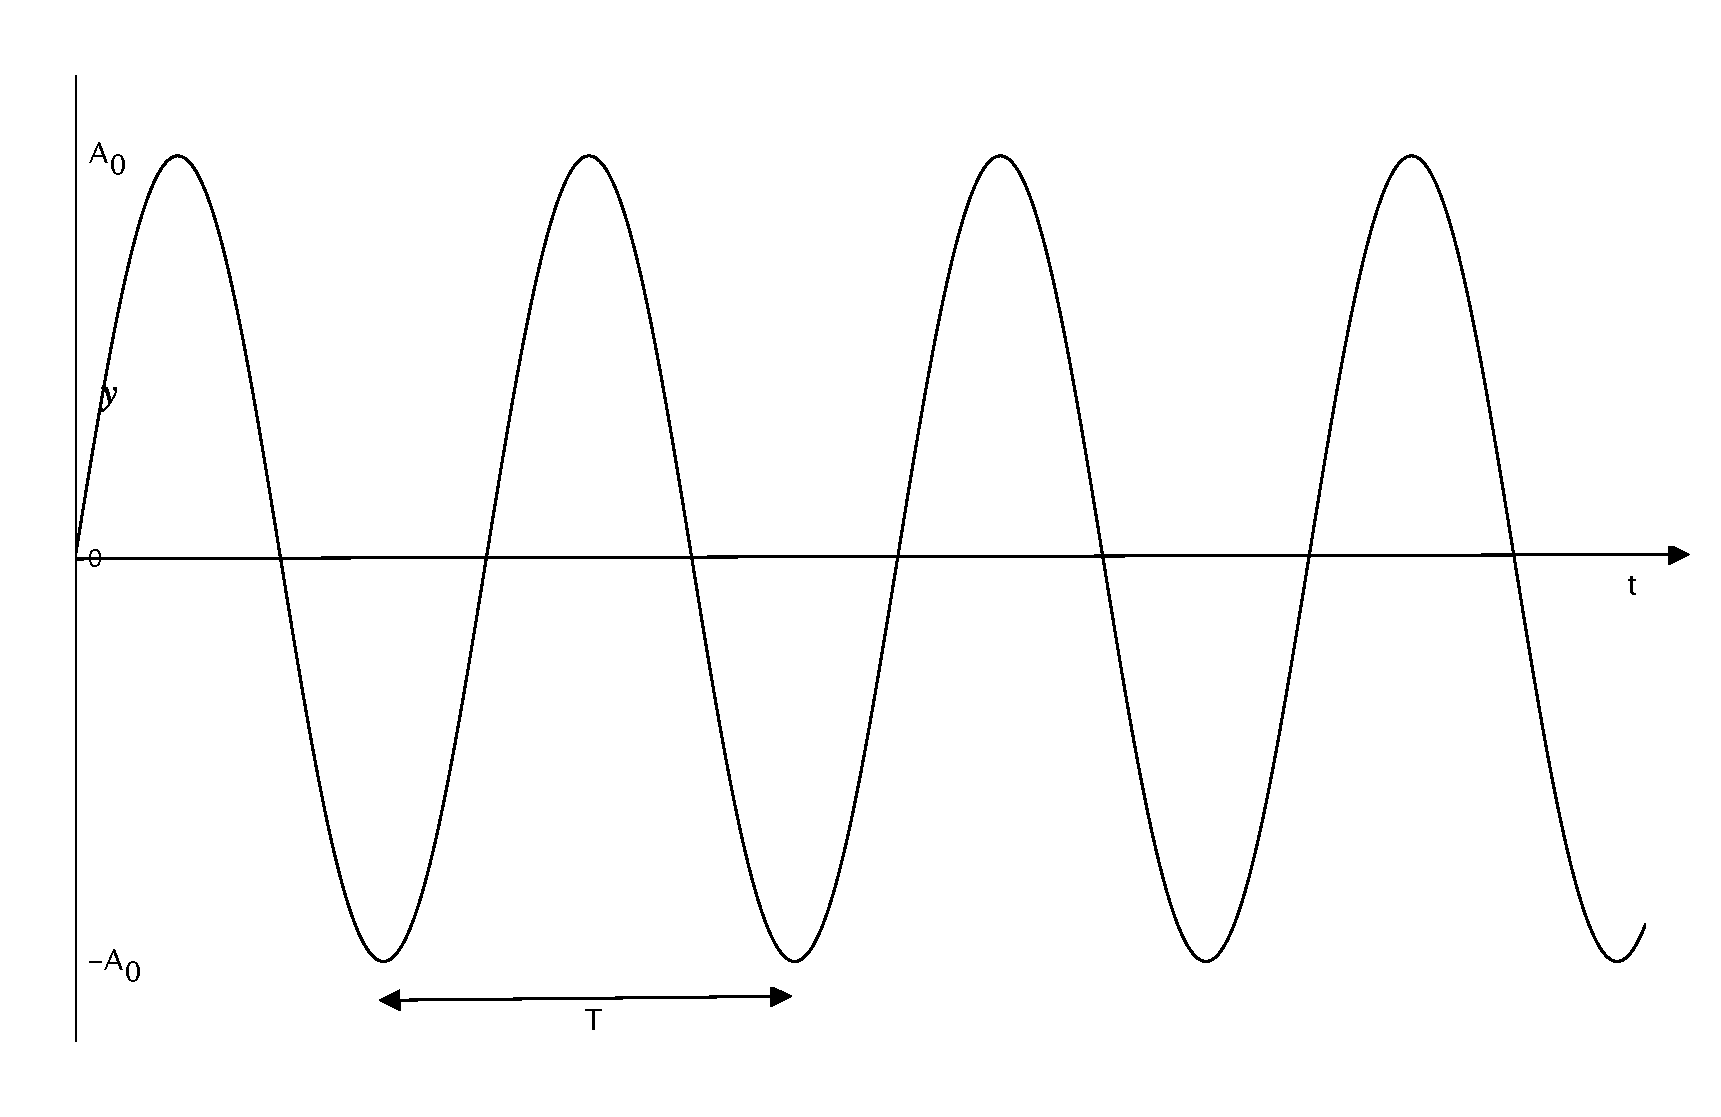
\includegraphics[width=0.6\textwidth]{sinus} \caption{Sinal correspondente a um som puro\label{fig:1} } 
\end{figure}


O exemplo mais conhecido de um oscilador que emite numa só  frequência é o diapasão. 
Contudo os sons agradáveis que ouvimos no dia a dia, como a música, são composições mais ou menos complexas de múltiplos sinais de diferentes frequências e amplitudes. Uma simples nota musical emitida por um instrumento é um sinal periódico, mas não corresponde normalmente a uma só frequência pura. No entanto de acordo com a análise de Fourier qualquer sinal periódico pode ser decomposto numa soma de sinais puros de diferentes frequências. O sinal de frequência mais baixa chama-se a fundamental ou 1ª harmónica e os sinais de frequência múltipla da fundamental chamam-se harmónicas de 2ª, 3ª, ..., nª ordem. Como exemplo na figura \ref{fig:harm} está representado um sinal periódico e a sua decomposição nas quatro harmónicas que lhe estão associadas estando representado na figura \ref{fig:harm_spectrum} o espetro do mesmo sinal.

\begin{figure}
	[tbp] \centering 
	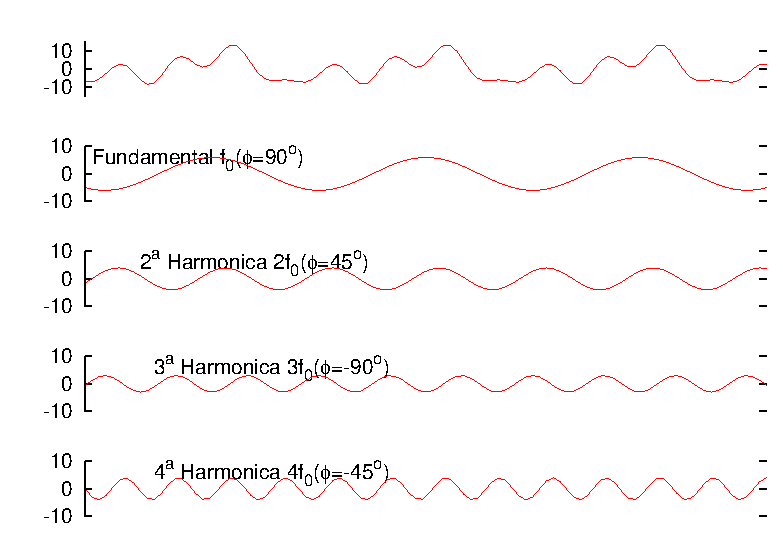
\includegraphics[width=0.8\textwidth]{harm} \caption{Sinal periódico composto por várias Harmónicas\label{fig:harm} } 
\end{figure}

\begin{figure}
	[htbp] \centering 
	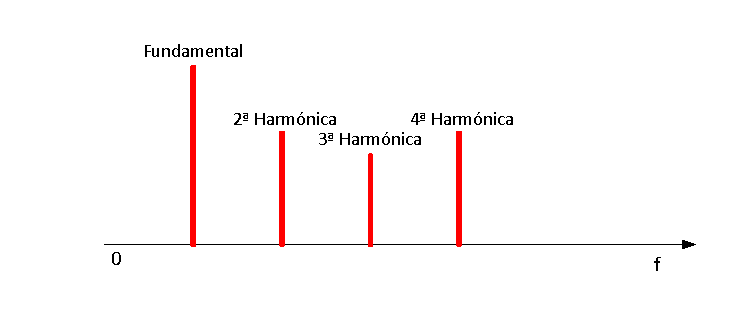
\includegraphics[width=0.7\textwidth]{harm_spectrum} \caption{Espetro de frequências do sinal da figura anterior\label{fig:harm_spectrum} } 
\end{figure}

% Na figura 4 estão representados como exemplos os espetros dos sinais acústicos emitidos pelas 
%cordas A e D de um violino quando o som fundamental tem uma frequência de 440 Hz. 

Os instrumentos musicais distinguem-se, entre outros atributos sonoros, pelo seu conteúdo espetral.
Nomeadamente notas acústicas idênticas tocadas por diferentes instrumentos musicais têm diferentes \emph{timbres}, pois embora a frequência da fundamental seja a mesma as intensidades das harmónicas dependem do instrumento e da forma como se tocam\footnote{Pode experimentar facilmente no seu computador com  com o programa “Audacity” (http://audacity.sourceforge.net), gravar um som de uma nota de instrumento musical e observar o seu espetro com comando: “Analyze Menu->Plot Spectrum”}.

%Como exemplo estão representados na figura 5 os sinais emitidos por quatro instrumentos diferentes quando cada um deles toca o dó central %(fundamental nos 256 Hz)

\subsection{\sf Perturbações com o caráter de onda}

Consideremos uma perturbação descrita pela grandeza y que se propaga ao longo do eixo sem se deformar com uma velocidade $v$ de acordo com a representação esquemática evidenciada na figura \ref{fig:Propag_onda}\footnote{Uma perturbação desse tipo pode ser facilmente obtida com uma corda esticada presa numa extremidade a qual se dá um impulso na outra extremidade com a mão que a sustenta.}.

\begin{figure}
	[tbp]  \centering 
	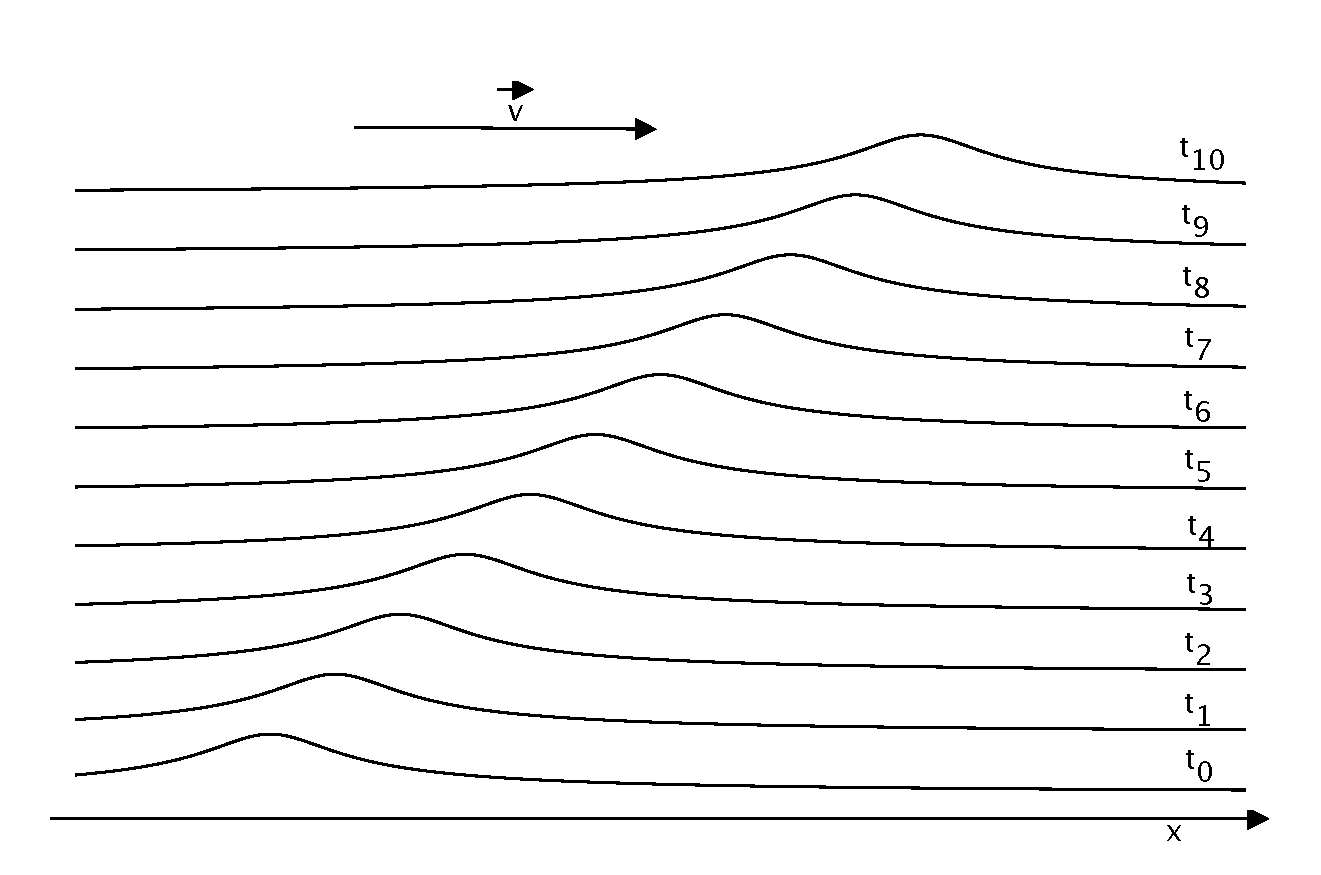
\includegraphics[width=0.7\textwidth]{Propag_onda} \caption{Perturbação que se propaga no espaço\label{fig:Propag_onda}} 
\end{figure}

Facilmente se compreende que a perturbação $y$ pode ser descrita por uma equação do tipo:

\begin{equation}
	\label{eq:onda}
y=f(x- vt)	
\end{equation}

Sendo fácil de verificar que a função (\ref{eq:onda}) obedece à identidade:

\begin{equation}
	\label{eq:onda2}
	\frac{\partial^2 f}{\partial x^2} = \frac{1}{v^2}  \frac{\partial^2 f}{\partial t^2} 
\end{equation}

que é conhecida com a designação de equação de onda da perturbação\footnote{Na propagação a 3 dimensões esta equação escreve-se com ajuda do operador laplaciano:
 $\Delta f = \nabla^2 f = \nabla \cdot \nabla f = \frac{1}{v^2} \;  \frac{\partial^2 f}{\partial t^2} 
\Leftrightarrow  \frac{\partial^2 f}{\partial x^2} +  \frac{\partial^2 f}{\partial y^2} +  \frac{\partial^2 f}{\partial z^2} =  
\frac{1}{v^2} \;  \frac{\partial^2 f}{\partial t^2} $}. 

Qualquer grandeza, $f$, que obedeça a uma equação do tipo (\ref{eq:onda2}) tem associado um caráter ondulatório. É o caso das ondas mecânicas e eletromagnéticas (e.g. Rádio, Luz, UV, etc.).

O exemplo simples apresentado no parágrafo anterior serviu para ilustrar que uma grandeza com caráter ondulatório tem uma dupla dependência no tempo e no espaço e é traduzida por uma função do tipo $f(x-vt)$. Contudo em muitos dos casos do dia a dia as perturbações emitidas têm um caráter periódico. Tal é o caso de uma sirene que  emite um sinal audível de frequência, $Freq = 1/T$, que indica o meio dia num quartel de bombeiros ou avisa os barcos da proximidade da terra num dia de nevoeiro, o som de um diapasão ou  uma orquestra quando afina pela nota Lá ($Freq_{La} = 440\, Hz$). 

Se considerarmos uma direção $x$ segundo a qual o sinal se propaga deveremos ter uma representação espacial do tipo da evidenciada na figura \ref{fig:propag_esp}, sendo $\lambda$ o comprimento de onda que depende do meio onde a onda se propaga.


\begin{figure} [!htbp] 
	\centering 
	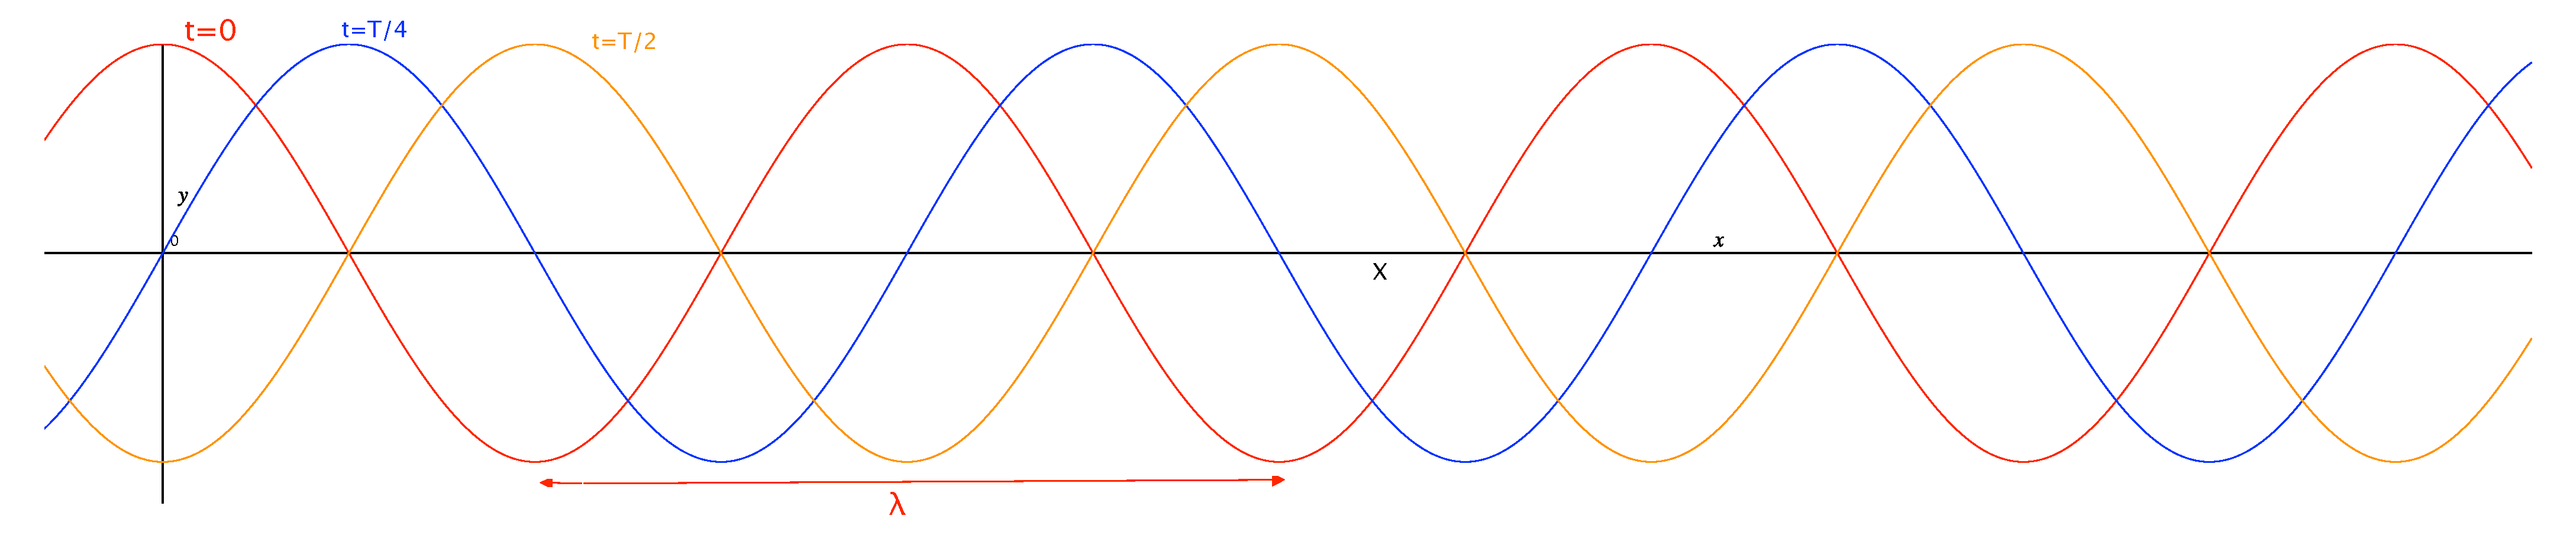
\includegraphics[width=0.7\textwidth]{propag_esp} 
	\caption{\label{fig:propag_esp}} 
\end{figure}

Na figura \ref{fig:propag_tempo} está evidenciada uma representação temporal da mesma perturbação para três valores diferentes de $x$. Nesta representação $T$ é o período de oscilação que é uma caraterística do emissor, não dependendo do meio. É fácil de verificar que a perturbação representada nas figuras \ref{fig:propag_esp} e \ref{fig:propag_tempo} é descrita por uma equação do tipo (\ref{eq:onda}) que no caso presente toma a forma\footnote{Aqui, para simplificar admite-se desprezável a atenuação na amplitude. $A(t)=$constante}:

\begin{figure} [!htbp] 
	\centering 
	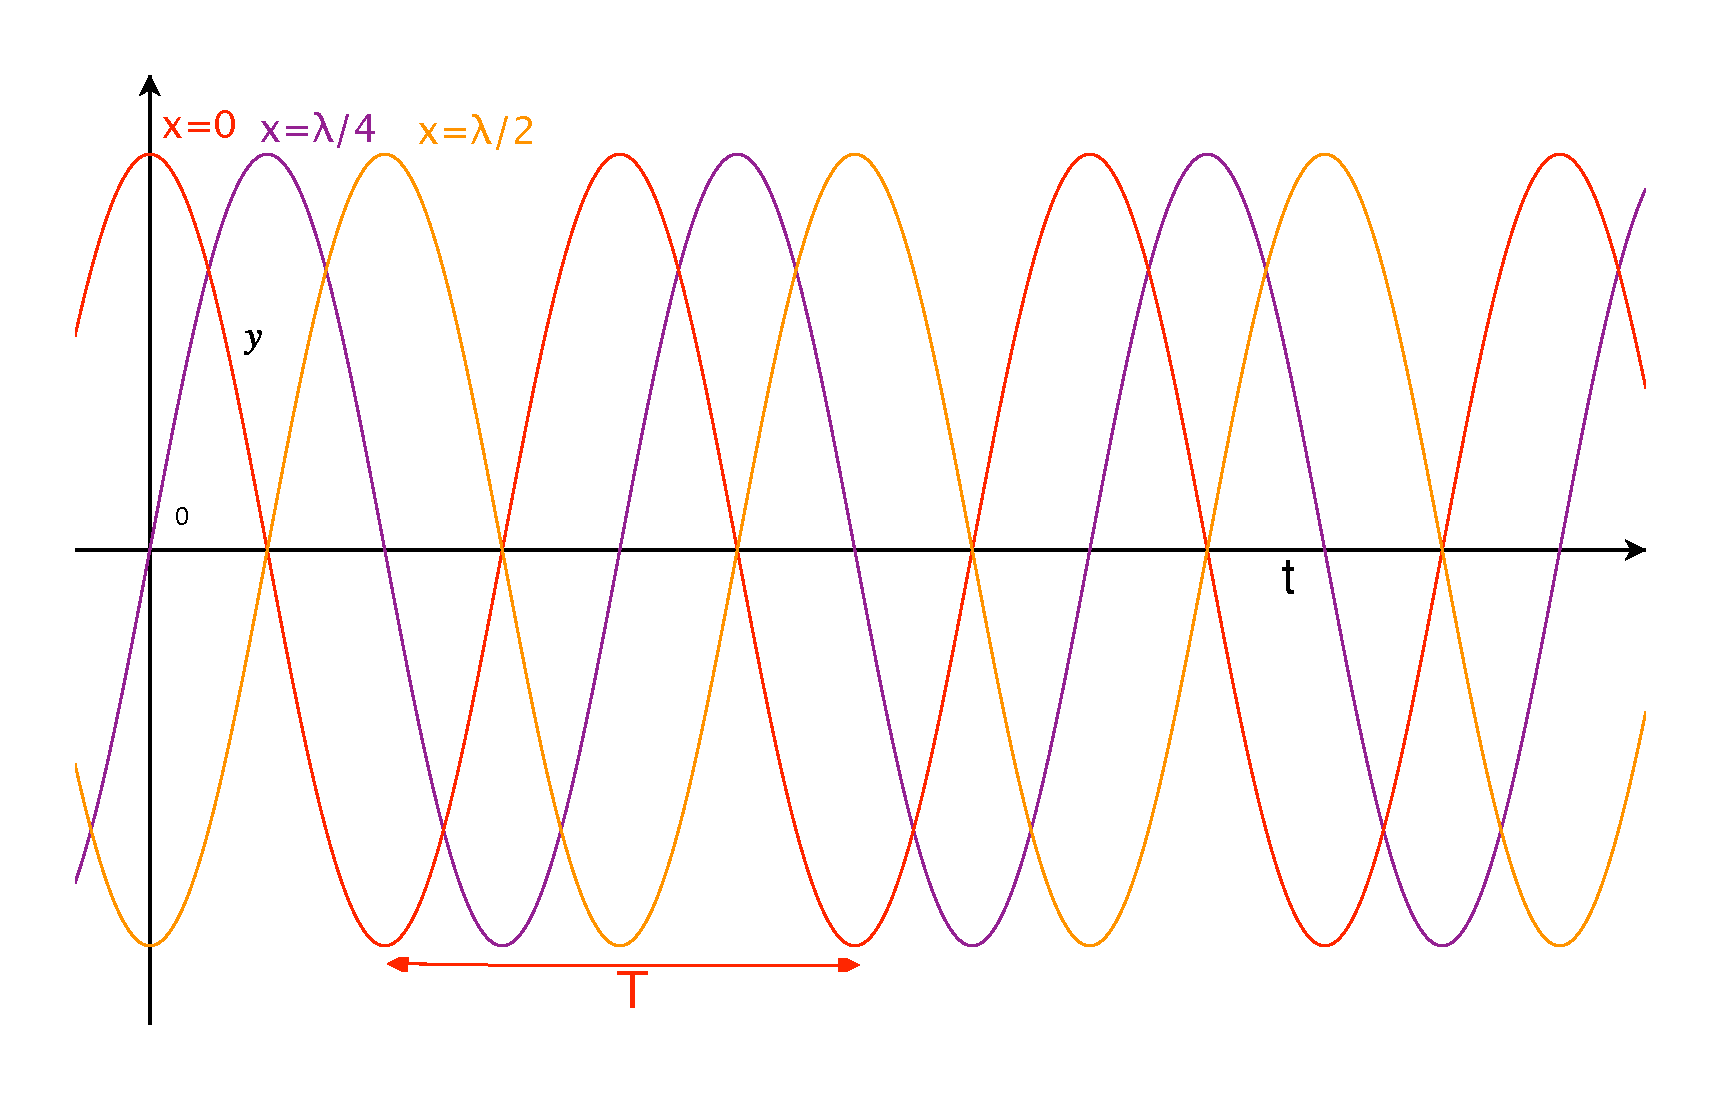
\includegraphics[width=0.7\textwidth]{propag_tempo} 
	\caption{\label{fig:propag_tempo}} 
\end{figure}

\begin{equation}
	\label{eq:onda3}
	y= A_0 \cos  \left(\frac{2\, \pi }{\lambda} x - \frac{2\,\pi }{T}\, t  \right) = 
	 A_0 \cos  \left( \frac{2\, \pi }{\lambda} (x- v\,t)  \right) 
\end{equation}


Sendo $v=\frac{\lambda }{T}$ a velocidade de propagação da perturbação\footnote{Velocidade de fase,  $v=\frac{\omega}{k} = \frac{\lambda}{T}$, que pode variar com a frequência. Quando o sinal contém várias frequências é necessário utilizar o conceito de velocidade de grupo}, $\omega=\frac{2\, \pi }{T}$ a \emph{frequência angular} e $k=\frac{2\, \pi }{\lambda}$ o \emph{número de onda}.

\subsection{\sf Velocidade de Propagação}

A velocidade de propagação de uma onda sonora longitudinal, que é uma perturbação da pressão local,  num fluido (ar ou água, por exemplo) é dado pela expressão:   
\begin{equation}
	\label{eq:veloc}
	v = \sqrt{\frac{K}{\rho}}
\end{equation}
em que $K$ é o módulo volúmico de compressão, “bulk modulus” $\Delta P= K \frac{\Delta V}{V}$ e $\rho$ a densidade volúmica. Para um gás como o 
ar seco (0\% de humidade) $K$ é proporcional à pressão, que por sua vez depende da densidade e temperatura absoluta.

Como as variações de pressão são muito rápidas para ocorrer transmissão de calor, considera-se uma variação de pressão \emph{adiabática} e $v$ é dado por 
\begin{equation}
	\label{eq:veloc2}
	v = \sqrt{\frac{\gamma\,R\,T}{M}}
\end{equation}
em que $R=8.314\,J\,K^{-1}\,mol^{-1}$ constante dos gases perfeitos, $M$ a massa molar média do gás e, $\gamma \equiv \frac{C_p}{C_v}$, a Constante Adiabática, tendo $C_p$ como Calor específico a {\bf pressão constante} e $C_v$ como Calor específico a {\bf volume constante}.

Para o ar seco, cujos $98\%$ são constituídos por moléculas diatómicas, tem-se $M_{ar}=29\times 10^{-3}\,Kg/mol$ e $\gamma_{ar} \simeq1.4$ e $v{ar} = (331.3 + 0.606 \cdot \Theta)$, com $\Theta)$  em graus centígrados, $ºC$.

\subsection{\sf Nível Sonoro}
O nível sonoro que está relacionado com a amplitude da variação da pressão  da perturbação, $\frac{\Delta p}{p}$\footnote{Esta variação é contudo muito pequena: uma variação $\Delta p=1\,Pa$ para uma atmosfera $p= 101323\,Pa$ já pode causar danos no ouvido ($L_p = 94\,dB$)}. Como o ouvido humano 
não tem uma resposta linear e abrange uma gama muito grande de amplitudes é habitual designá-lo pelo nível de pressão acústica (“Sound Pressure Level-SPL”), dado em \emph{decibéis}, pela expressão:

\begin{equation}
	\label{eq:n_sonoro}
	L_p = 10 \log_{10} \left( \frac{(\Delta p_{ef})^2}{p_{ref}^2} \right) = 20 \log_{10} \left( \frac{\Delta p_{ef}}{p_{ref}} \right)  \; \; dB
\end{equation}

Neste caso, $\Delta p_{ef}$, é o valor eficaz (RMS) da variação de pressão e $p_{ref}$ um valor de referência,  $p_{ref}=20\, \mu  Pa$ no ar, considerado como o limiar mínimo da audiçao humana ($L_p = 0\,dB$). Uma só “Vuvuzela” a 1 metro de distância pode provocar um nível sonoro de $L_p = 120\,dB$.


\newpage
\section{\sf Procedimento Experimental}
\subsection{\sf Material utilizado}

\begin{enumerate}
\item Tubo acústico de comprimento variável equipado com altifalante e microfone. 
\item Gerador de sinais. Osciloscópio. Cronómetro. 
\item Dois diapasões e microfone. Bobina com núcleo de ferro. 
\item Termómetro. 
\end{enumerate}

\subsection{\sf Velocidade de propagação do som no ar}
Ligue o altifalante a um gerador de sinais, com um sinal \emph{retangular}, de modo a criar impulsos sonoros com uma taxa de cerca de 20 impulsos por segundo.
Utilize a escala de tempo mais adequada e o circuito de \emph{Trigger} em Modo “NORMAL”, com disparo pelo canal ligado ao gerador de sinais(CH1).  
Obtenha no osciloscópio a vibração caraterística do altifalante (copiando-a para o relatório) de um impulso sonoro e estime a sua frequência fundamental.  

Meça, usando o osciloscópio, o tempo necessário para um impulso sonoro, percorrer uma certa distância (tubo acústico de comprimento variável).
Faça um número suficiente de medidas, utilizando toda a gama distâncias permitidas pelo tubo. Obtenha a partir de uma representação gráfica, a estimativa da velocidade de propagação do som no ar e a incerteza. Leia a temperatura da sala. Obtenha uma estimação da precisão da determinação, assim como o desvio à exactidão. 

\subsection{\sf Frequência de ressonância do diapasão}
\subsubsection{\sf Medida direta do período}
Meça, usando o osciloscópio, o período da vibração de ressonância do diapasão excitado por percussão. Faça observações com pelo menos 2 valores diferentes da base de tempo e para cada um deles, escolha as condições de maior precisão. Estime a incerteza do período. Calcule a frequência e a incerteza associada. Estime o desvio à exactidão. Repita para um segundo diapasão. 
\subsubsection{\sf Medida por comparação}
Utilize um gerador de sinais e o osciloscópio sem a base de tempo (Modo “XY”), para
medir a frequencia ressonância dos 2 diapasões, atravéz das figuras de Lissajous.
%Como devia proceder para determinar a referida frequência com maior precisão, com o equipamento de que dispõe no laboratório? Execute e prove experimentalmente. Estime a precisão das determinações, assim como a exactidão obtida com este método e compare com o anterior. 
\subsubsection{\sf Medida por excitação da frequência de ressonância }
A excitação do diapasão pode ser feita por indução electromagnética. Usando uma bobina com núcleo de ferro, à qual é aplicada uma tensão alternada sinusoidal, tente seleccionar o valor da frequência da tensão capaz de excitar o diapasão.
\subsubsection{\sf Medida do limite da audição}
Utilizando o gerador de sinais ligado ao  altifalante, com um sinal \emph{sinusoidal}, determine a frequência máxima que consegue ouvir.

\subsection{\sf Amortecimento da vibração sonora}

A amplitude do sinal sonoro produzido pelo diapasão percutido vai diminuir exponencialmente no tempo (devido à perda da energia mecânica do diapasão, por devido ao atrito do ar e  emissão de potência sonora). A dependência no tempo dos valores dessa amplitude $A_{max}(t)$  pode ser descrita pela expressão $A_{max}(t) = A_0 \; e^{-\lambda\,t}$. A amplitude do sinal detectado pelo microfone que é observada no osciloscópio segue a mesma evolução no tempo. 
Utilize de preferência o osciloscópio sem a base de tempo (Modo “XY”), com o microfone ligado ao canal \emph{vertical} e utilizando o máximo da escala para medir a amplitude. Considere p.ex. $A_{max}(0) = 7\,div$, (início da contagem de tempo) e em sucessivos ensaios meça o tempo necessário para a amplitude diminuir até  $A_{max}(t_i) = 6,\,5,\,4,\,3,\,2,\,1\,div$.

Observe essa evolução para dois diapasões diferentes.
Usando uma representação gráfica adequada (e.g. gráfico semi-logaritmíco) da função $A_{max}(t)$  faça uma estimativa do coeficiente de amortecimento, $\lambda$, e a respectiva incerteza.

\end{document} 	

